\section{CLI for Libraries}

\begin{frame}[fragile]{\secname}
  \textbf{Use-Cases}
  \begin{itemize}
    \item Use CI to make sure all library elements are valid
    \item Check pull requests for library convention violations (ToDo)
  \end{itemize}

  \bigskip

  \textbf{Usage}
  \small
  \begin{minted}[baselinestretch=.8,style=perldoc]{console}
$ librepcb-cli open-library --all --strict MyLibrary.lplib
Open library 'MyLibrary.lplib'...
Process 86 component categories...
Process 44 package categories...
Process 37 symbols...
Process 492 packages...
Process 34 components...
Process 37 devices...
SUCCESS
  \end{minted}
\end{frame}


\begin{frame}{\secname}
  \begin{center}
    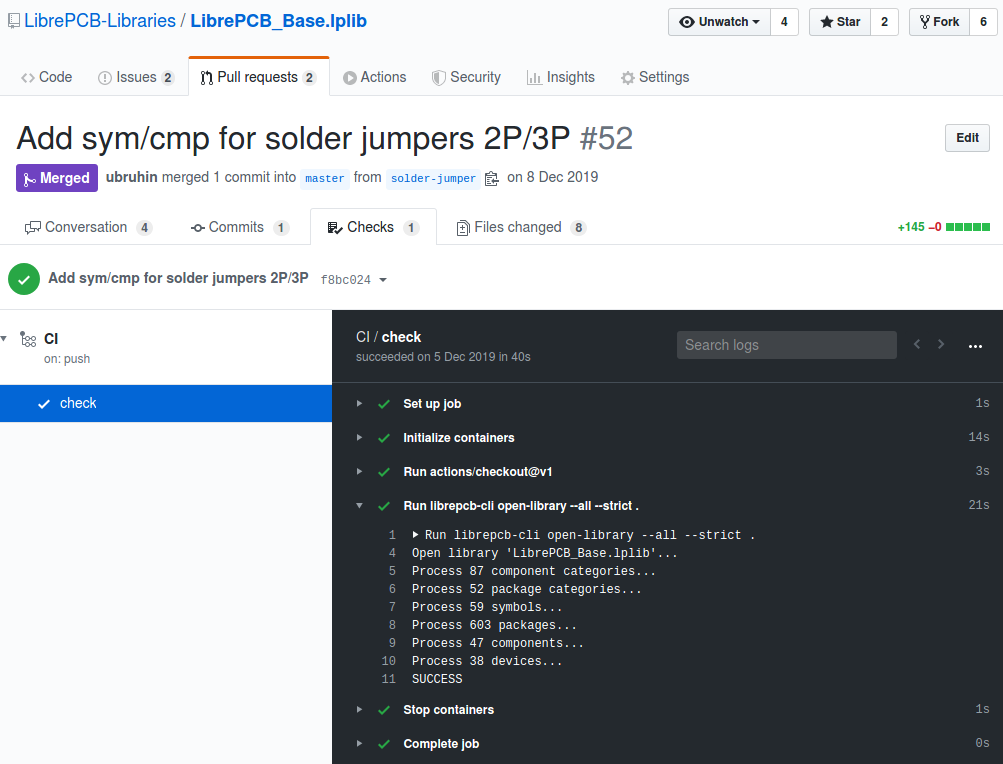
\includegraphics[width=0.9\textwidth]{images/cli_libraries_github.png}
  \end{center}
\end{frame}
